\documentclass[conference]{IEEEtran}   	% use "amsart" instead of "article" for AMSLaTeX format
\usepackage{geometry}                		% See geometry.pdf to learn the layout options. There are lots.

\usepackage{graphicx}				% Use pdf, png, jpg, or eps§ with pdflatex; use eps in DVI mode
\usepackage{array}
\usepackage{cite}
\usepackage{hyperref}


\title{An experimental platform for home wireless router}
\author{Xuefeng Huang}

\begin{document}
\maketitle
\begin{abstract}
As one of the most economically significant and fastest growing sectors of the Internet, broadband networks have attracted interest from researchers. To better understand broadband networks, we developed Seattle, an open research and educational testbed that utilizes computational resources provided by end users on their home wireless routers with custom firmware (OpenWrt\cite{openwrt}). Unlike most other platforms, Seattle provides a privacy protection of embedded device data and maintains the security of donated device from potentially buggy experiment codes. We find that our platform is flexible enough to implement a variety of network measurements despite its security restrictions. This paper discusses some of the challenges we faced building and using a platform for deploying measurement in home networks, describe its design and implementation.
\end{abstract}
%\section{}
%\subsection{}
\section{Introduction}
Currently it has been difficult to study home networks on a large scale because network technologies like network address translators (NATs) present only an opaque view of the home network to the global Internet. To better understand home networks, an experimental platform should be hosted in home networks, to provide visibility into the missing part of Internet. While previous works\cite{183951} have studied access networks from home gateway, they are unable to let researchers run arbitrary codes without compromising the privacy of the user and abuse of host or network resources. We present Seattle, a platform for measurement experimentation from home gateway. Seattle is able to deploy in home wireless router so that it is capable of running both active and passive experiments from a vantage point between the access ISP and the home network, as shown in Fig. 1.
\newline
In this paper, we introduce Seattle Testbed\cite{cappos2009seattle}, a distributed cloud platform that allows researchers to run their project on system worldwide. This testbed provides secure data access while preserving user privacy. Through a programmable interface on device, the testbed enables researchers to deploy a wide range of network measurements. We also discuss the constraints we faced in the design, implementation and deployment of Seattle.

\begin{figure}%[h]
\centering
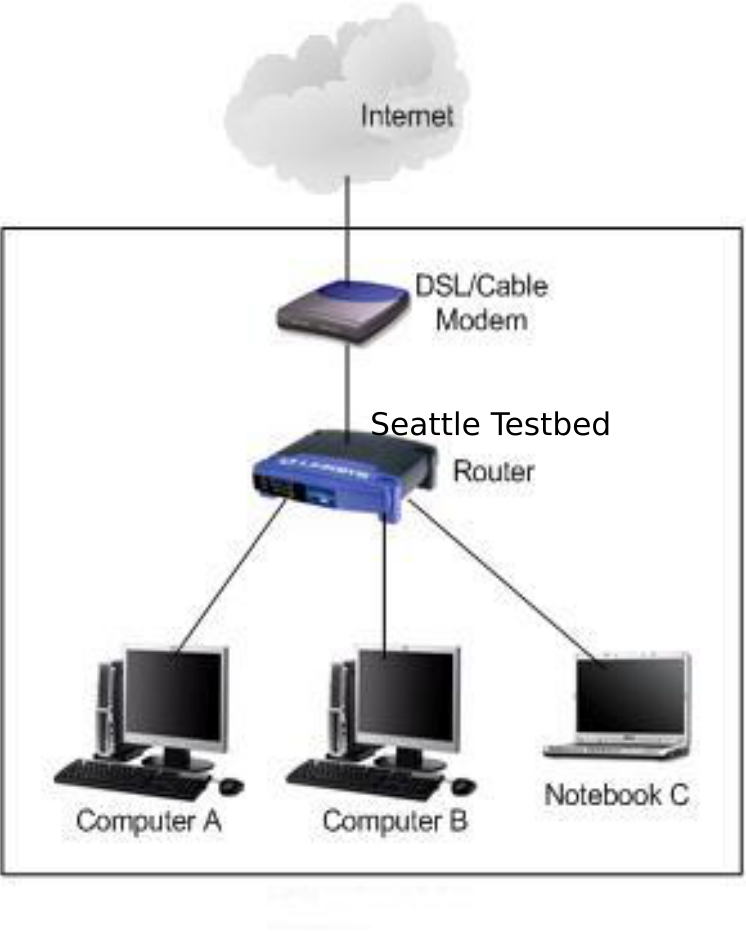
\includegraphics[width=0.5\columnwidth]{home-network.jpg}
\caption{The router sits directly behind the modem in the home network.}
\label{figure:design}
\end{figure}

\section{CHALLENGES}
\label{sec.challenges}
A testbed that allows researchers to execute code across donated embedded devices faces four major challenges: 
\begin{itemize}
\item First, the embedded devices poses a limited resources challenge. It is hard to run heavy scripting languages like Python or Ruby. 
\item The second challenge is user's networking experience. Seattle nodes are on the direct path of real Internet users. A malicious network measurement experiment will noticeably affect a normal user's network experience. 
\item The third challenge is secure data access. Network traffic data pose a risk to device donors whose devices are exposed to malicious code written by users. 
\item The fourth challenge is data privacy. Users should not gain access to information that donors don't want to share.
\end{itemize}
As the development of hardware technology and based on our practical experience, running Python codes are going well on embedded devices. And the last three challenges can be solved via using a secure and performance-isolated sandbox and a reference monitor framework we proposed.

\section{Contributions}
\label{sec.contributions}
\textit{1) Home routers platform:} This platform is based on Seattle\cite{zhuang2013experience}, a community-driven, open-source cloud computing system. Compared to computer and mobile device environments, deployment on home wireless router has more resource limitation such as restricted computational resources. However, recently we are able to port Seattle to embedded devices. Users can build their own Seattle installer (IPK) via config file we provide using OpenWrt SDK and install it on the device directly. Currently, I deploy this platform in TP-Link TL-WDR3600 router, which has a 560 MHz MIPS processor, 8MB of flash storage, 128MB of RAM and a dual-band wireless interface.
\newline

\textit{2) Extensions to Seattle Testbed:}  Our testbed implements new research capabilities for home wireless router by improving on the Seattle sandbox. To handle home wireless routers, our testbed uses low-level system calls in the OpenWrt platform\cite{openwrt} with the Restriction Python (Repy)\cite{cappos2010retaining}, the core sandbox of Seattle. In order to securely interact with home routers on remote user devices, we use Fence~\cite{li2015fence} to allocate a fixed percentage of the device's CPU, memory disk, and other resources to one or more VMs. For example, we set the legal times of accessing proc file system to prevent DoS attack using our API calls. Our testbed adds seven functionalities based on Repy, as shown in in Table I. Through these new functionalities I proposed, researchers are able to implement a wide range of network measurements, as shown in in Table II.
\newline

\begin{table*}
\scriptsize
\centering
\begin{tabular}{|p{.2\textwidth}| p{.4\textwidth}| m{.6\textwidth}|}
\hline
\textbf{API}    &  \textbf{Description} \\
 \hline
 {\bf scan} & {\bf Collect the list of access points found with a WiFi scan. For each access point we collect BSSID, SSID, signal strength and channel number.} \\
\hline
 {\bf get\_station} & {\bf Record downlink statistics per associated client (e.g., Total packets sent, received, retried, client's signal strength at home wireless router).} \\
\hline
 {\bf get\_network\_interface} & {\bf Return a list of available network interfaces.} \\
\hline
 {\bf get\_network\_bytes} & {\bf Record information about the configured network interfaces. The statistics include metrics such total number of received or transmitted bytes, drops, errors.} \\
\hline
 {\bf get\_network\_packets} & {\bf Record information about the configured network interfaces. The statistics include metrics such total number of received or transmitted packets, drops, errors.} \\
\hline
 {\bf ping} & {\bf A pure python ping implementation using raw sockets.} \\
\hline
 {\bf traceroute} & {\bf Return the route packets take to network host. } \\
\hline
\end{tabular}
\caption {New API }
\label{table:api_design}
\end{table*}

\begin{table*} 
\scriptsize
\centering
\begin{tabular}{|p{.1\textwidth}| p{.3\textwidth}| m{.2\textwidth}|}
\hline
\textbf{Type} & \textbf{Parameters} & \textbf{Descriptions} \\
 \hline
 {\bf Passive} & {\bf Aggregate traffic statistics per associated client (e.g., Total packets sent, received, retried,
client\'s signal strength at AP)\newline neighboring APs information} & {\bf Home network characteristics \newline Usage characteristics} \\
\hline
 {\bf Active} & {\bf Throughput, Latency, Loss, Jitter, traceroute, DNS lookups} & {\bf ISP characteristics \newline Internet connectivity and reachability} \\
\hline
\end{tabular}
\caption {Experiments obtained from Seattle}
\label{table:experiment}
\end{table*}

\textit{3) Experimental Characterization of home wireless networks: } By integrating Seattle with the home network, we get the benefits of a real world deployment while ensuring flexibility to run experiments without compromising home network. We demonstrate Seattle's utility by implementing one example usage case that together exercise different new API calls (get\_network\_bytes, get\_network\_interface, get\_station): monitoring how busy the WiFi channels in a place over one or two weeks. Our goal is to illustrate how Seattle can support disparate measurement needs.

\section{STATUS AND FUTURE WORK}
We have currently deployed Seattle in a router in the NYU lab. This device is added to Poly VLAN 147. Instead of traditional installer, Seattle is able to be installed via OPKG package manager\cite{opkg}\cite{seattle-openwrt}. It is better to resolve dependencies with packages in the repositories. In order to let Seattle group members test these new capabilities in home wireless router easily, I provided documentation and some example programs\cite{test}. Currently. those new API calls work fine from group members' feedback. I am currently studying the network traffic of home networks. Our plan is to analyze the periodicity of usage patterns in various home networks. The data we collect will include aggregated traffic information and timestamp. I have ran an experiment to collect data using Seattle in the home wireless router. However, due to the issue\cite{gettid_issue} about GETTID doesn't work in OpenWrt, I only can get aggregated traffic information.
\newline
In a few weeks, there are a few things I will work on:
\begin{itemize}
\item First of all, I will fix unsolved issue as mentioned above.
\item Secondly, I will demonstrate Seattle's utility in one study: monitoring how busy the WiFi channels in a place over one or two weeks. This experiment will take advantage of our new API calls and give researchers a good example to help them to write and launch their own measurements. 
\item Thirdly, writing a documentation for new API calls. 
\item Finally, I will finish my thesis before the deadline. I am currently writing my master thesis draft, it includes five sections: introduction, challenges and contributions, related work, a secure network testbed design, implementation. After obtaining actual experiment result, I will start working on evaluation and conclusion section. 
\end{itemize}  
If time is enough, I will work on integrating Seattle-OpenWrt package with Custom Installer Builder which is a tool for building and packaging Seattle base installers. Since creating an ipk file is different from creating a tarball, we should figure out a way to generate Seattle installer for OpenWrt using specified OpenWrt SDK automatically. 
\bibliographystyle{plain}
\bibliography{thesis}
\end{document}  